The evaluation was performed on a machine using two Intel(R) Haswell-EP Xeon(R) E5-2699v3 processors with total 36 cores supporting 72 threads. We use the latest
LLVM compiler version 3.8.0 for evaluating IOMP implementation. Test programs were designed to evaluate the overhead of these functions. 
%\subsubsection{{\sf omp\_quiesce}}

We first developed microbenchmarks for evaluating parallel startup cost after applying different wait policy or 
quiescing the runtime system, as well as the cost for the {\sf omp\_set\_wait\_policy} and {\sf omp\_quiesce} 
routines.  
Figure~\ref{omp:overhead_table} shows the results of the evaluation. 
The use of each of the two {\sf ACTIVE} policies and the PASSIVE(SPIN\_YIELD) policy 
introduce very minimum and neglectable overhead to the {\sf parallel} region startup. 
When PASSITVE(SUSPEND) policy is applied, we observed significant increase of overhead of creating parallel region, 
which can be explained by the cost to suspend and resume the runtime threas when the policy is in effect. 
The use of {\sf omp\_quiesce} with TERMINATE policy, which completely shutdown the 
runtime, dramatically increase the overhead, close to 1000x, of starting the a new parallel region. In this 
scenario, the cost of initializing the whole runtime is counted toward {\sf parallel} startup overhead. Second, 
for the overhead of the two routines, {\sf omp\_set\_wait\_policy} incurs very minimum overhead. The 
{\sf omp\_quiesce} routine however incurs high overhead since it needs to terminate the runtime threads as well as 
destroy all the resources allocated for the runtime (e.g. mutex, condition variables and memory, etc). 

%The overhead evaluations show that the ACTIVE(SPIN) and YIELD policies do not impact much of the {\sf parallel} 
%region start up. The PASSIVE(SLEEP) policies introduce overheads for creating new parallel regions that need to wake up sleeping thread, thus should use with care. The {\sf omp\_quiesce(KILL)} is a heavy operations and should only be
%used when there is no need to use the runtime in the program. 

%The test measures the overhead of starting 
%up an OpenMP runtime and shutting down a runtime by using {\sf omp\_quiesce}, as compared to creating a parallel region. 
%The cost of creating a parallel region is very light because of the use of internal hot teams maintained by the runtime. 
%The cost of shutting down the runtime is about half of the cost of starting a runtime, 
%but about 4 to 10 times of the cost of parallel region creation. 

\begin{figure}[ht]
    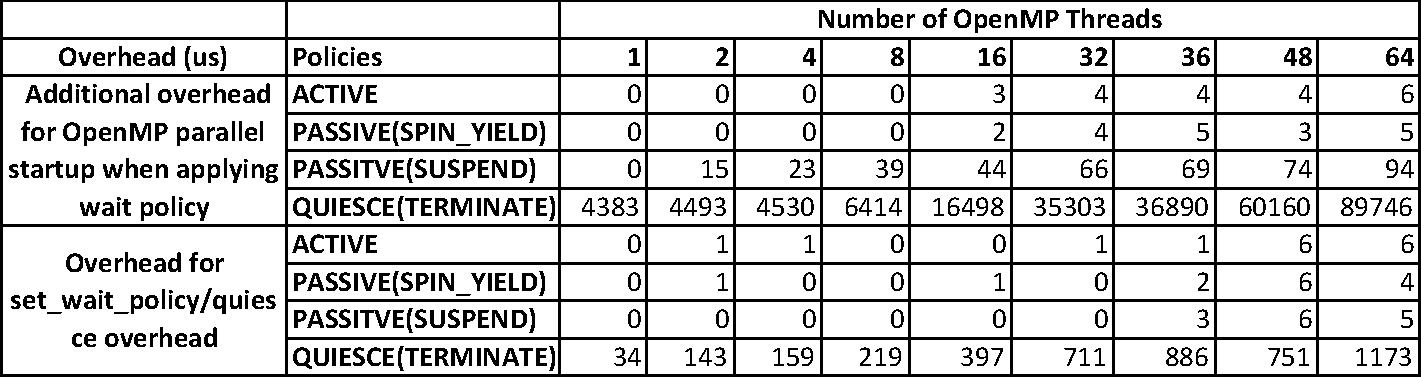
\includegraphics[width=0.99\textwidth] {images/parallel_set_quiesce_overhead}
    \caption{Overheads for OpenMP parallel and for {\sf omp\_set\_wait\_policy} and {\sf omp\_quiesce} implementation}
    \label{omp:overhead_table}
\end{figure}

\REM{
\begin{figure}[ht]
    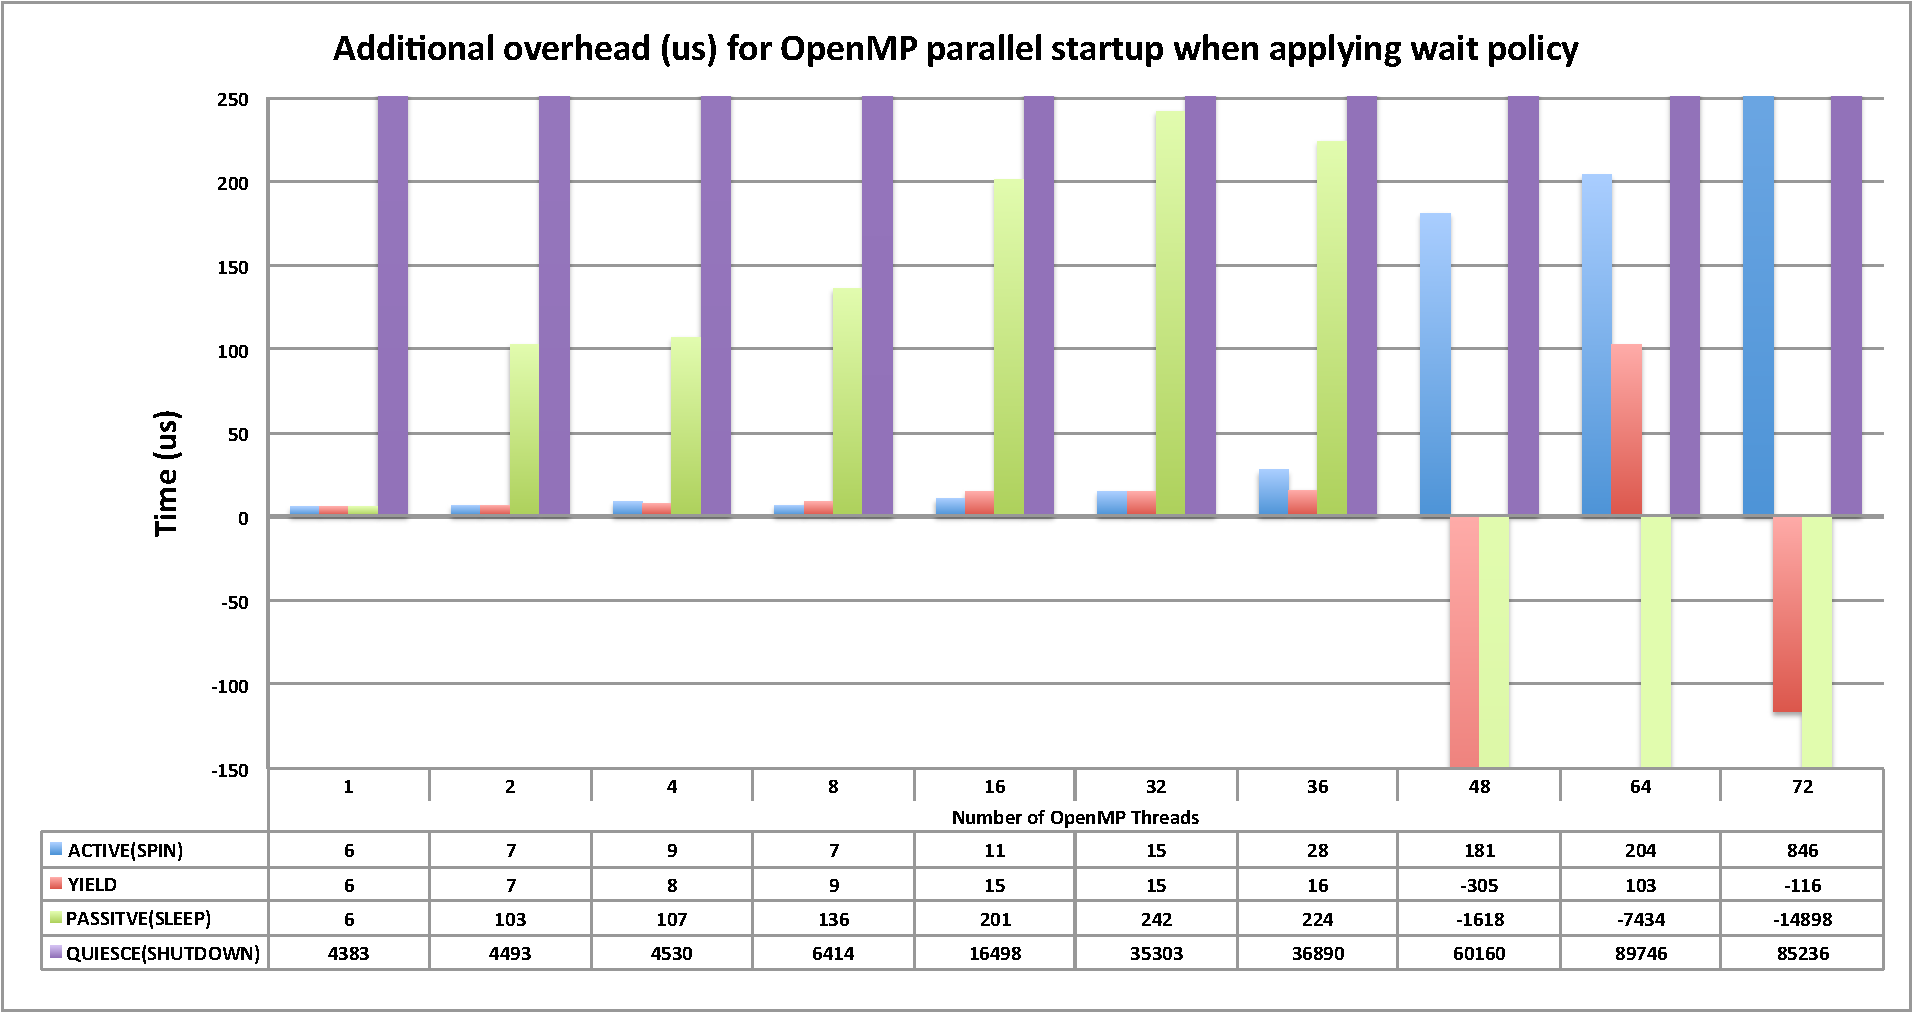
\includegraphics[width=0.99\textwidth] {images/parallel_overhead}
    \caption{Additional Overheads (us) for OpenMP parallel when applying {\sf omp\_set\_wait\_policy} and {\sf omp\_quiesce}}
    \label{omp:parallel_overhead}
\end{figure}
}

Our next evaluation was designed to measure the execution time of hybrid PThread/OpenMP program when different
wait policies are applied. We develop a program in which multiple PThreads are created, 
each of which executes the funciton shown in the following list. 
Each PThread first spins waiting for a specific period of time, and  
then enters into a parallel region in which perform busy-waiting for 3000 us.
The time periods of the two busy waiting (one is sequential and one is parallel) are carefully designed for
all PThreads so theoritically only one PThread enters into parallel region a time. The 
OpenMP threads for each PThread are scheduled by the kernel onto the available 
cores. When there are enough cores to support all threads (including the PThreads and OpenMP threads),
which means no oversubscription, mininum scheduling overhead and context switch are incurred, thus the optimal 
performance. In this test case, we define two crosspoints. The first crosspoint (\#1) is when the oversubscription
over the total number of cores in the test system (36 cores) happens and the second one (\#2) is when the oversubscription
over the total number of hardware threads (72) happends. 


\lstset{basicstyle=\sffamily\footnotesize,language=c, numbersep=1pt}
\begin{lstlisting}[frame=single]  % Start your code-block

void *omp_parallel_foo(void *ptr ) {   
    int user_thread_id = (int) ptr;
    for (int i=0; i<NUM_ITERATIONS; i++) {
        /* busy wait befor entering parallel region */
        busy_waiting(user_thread_id*3000);
#pragma omp parallel num_threads(num_ompthreads)
        {   
            busy_waiting(3000); /* act as computation */
        }
        omp_set_wait_policy(policy);
    }
}

\end{lstlisting}


\begin{figure}[h]
    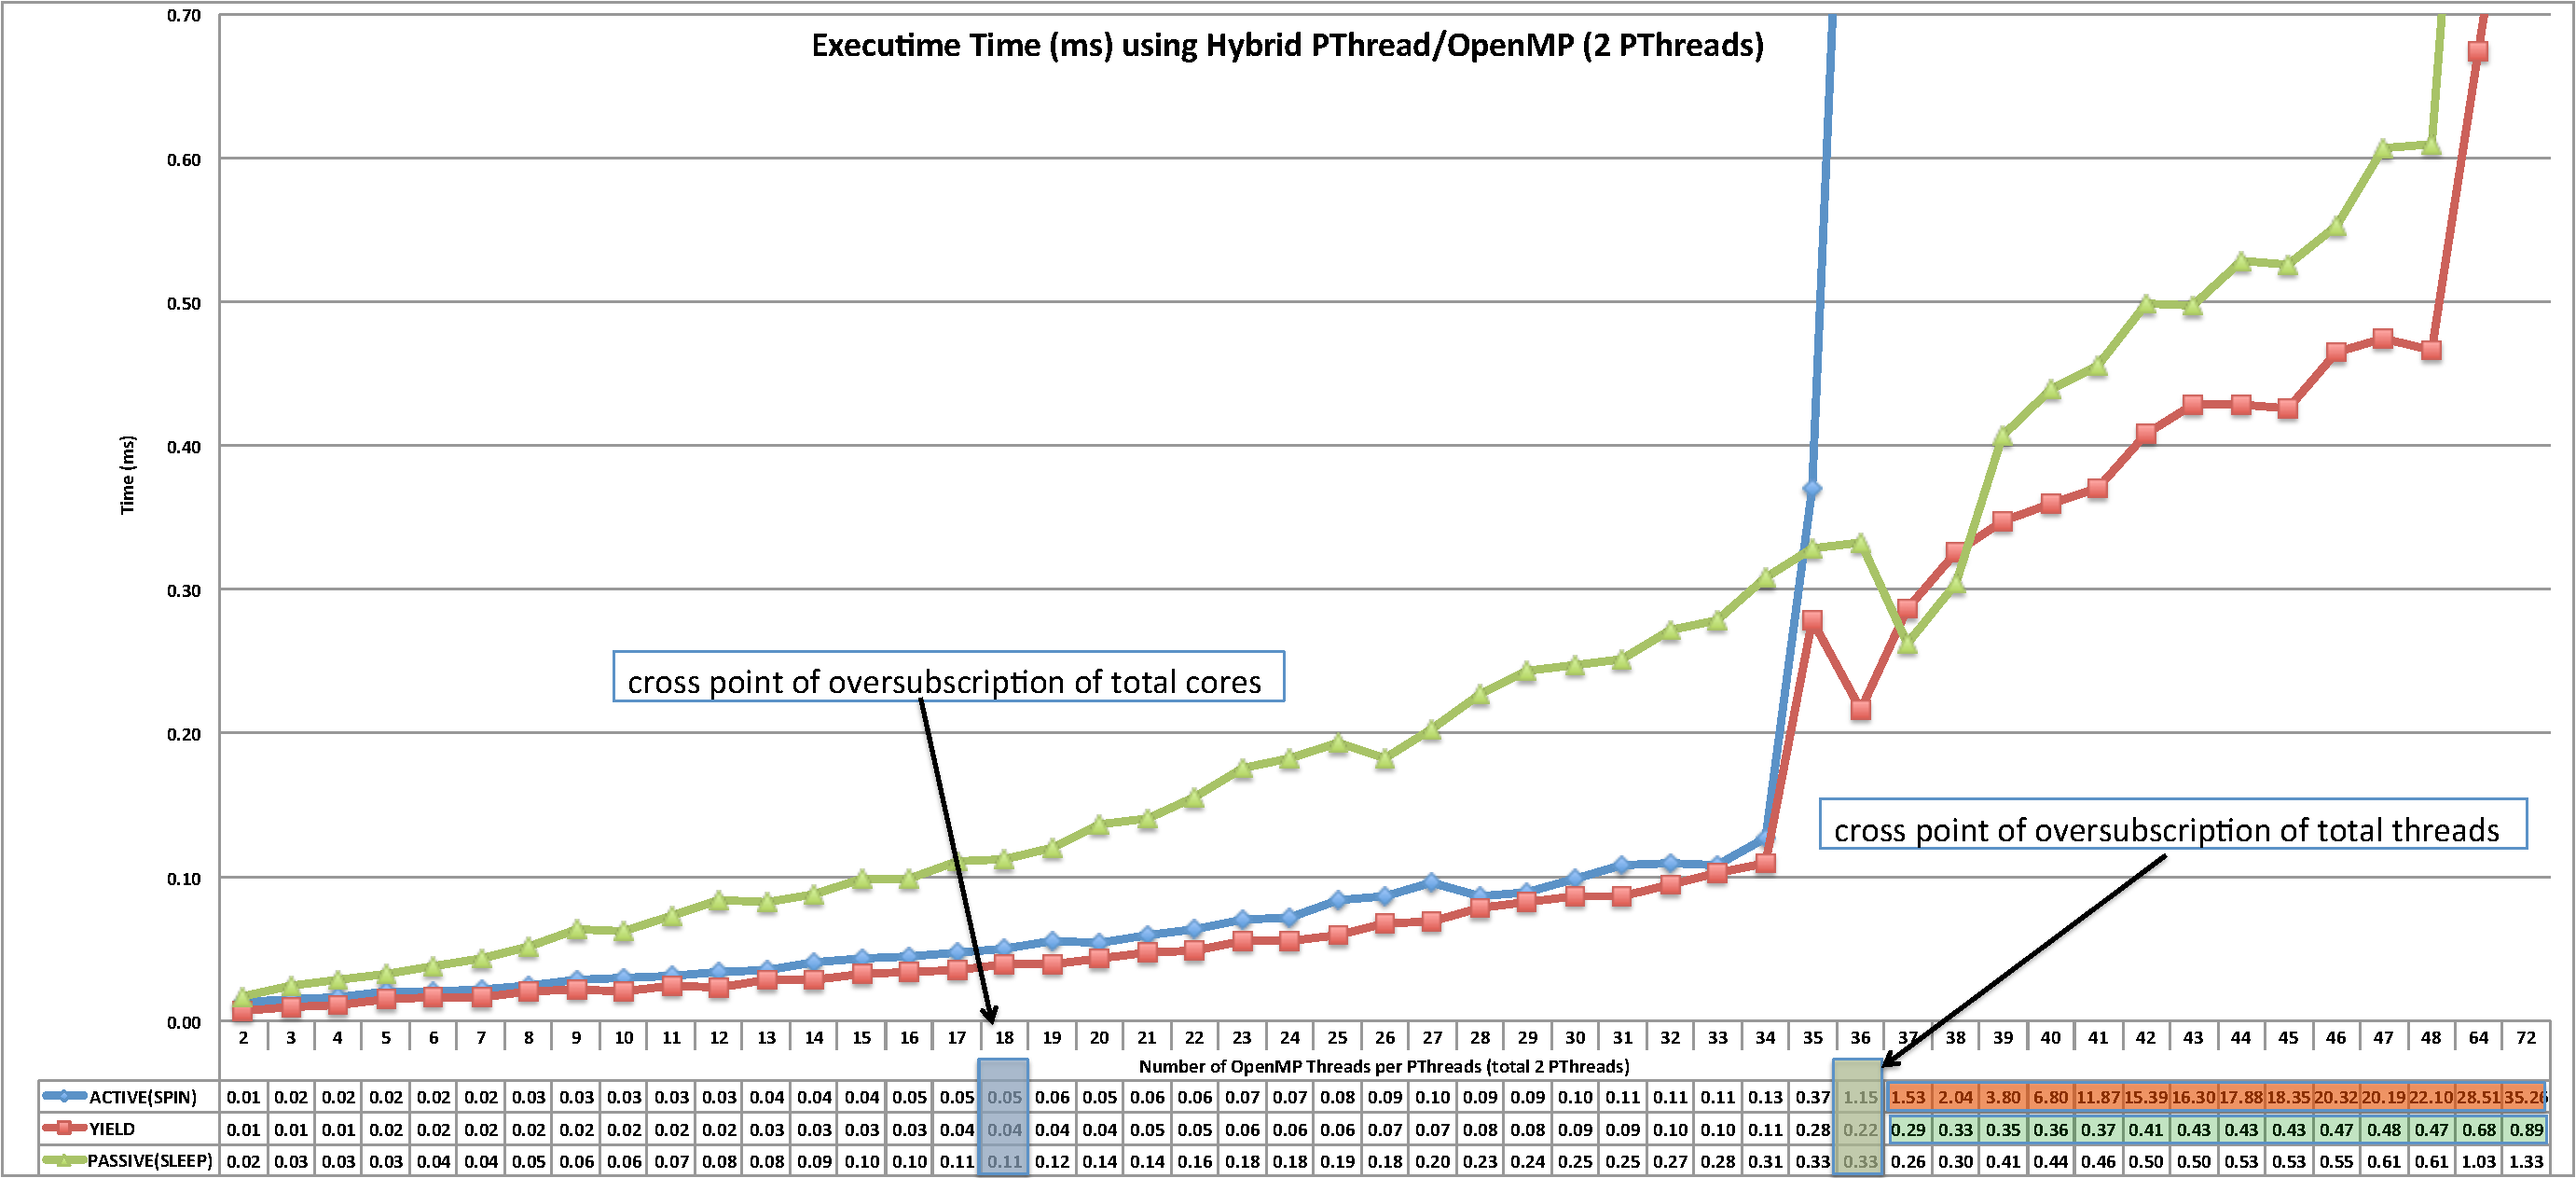
\includegraphics[width=0.99\textwidth] {images/2PThread_performance}
    \caption{Performance (ms) for hybrid PThreads/OpenMP execution: 2 PThreads and the system has total 36 cores for 72 threads.}
    \label{fig:2PThread_performance}
\end{figure}

\begin{figure}[h]
    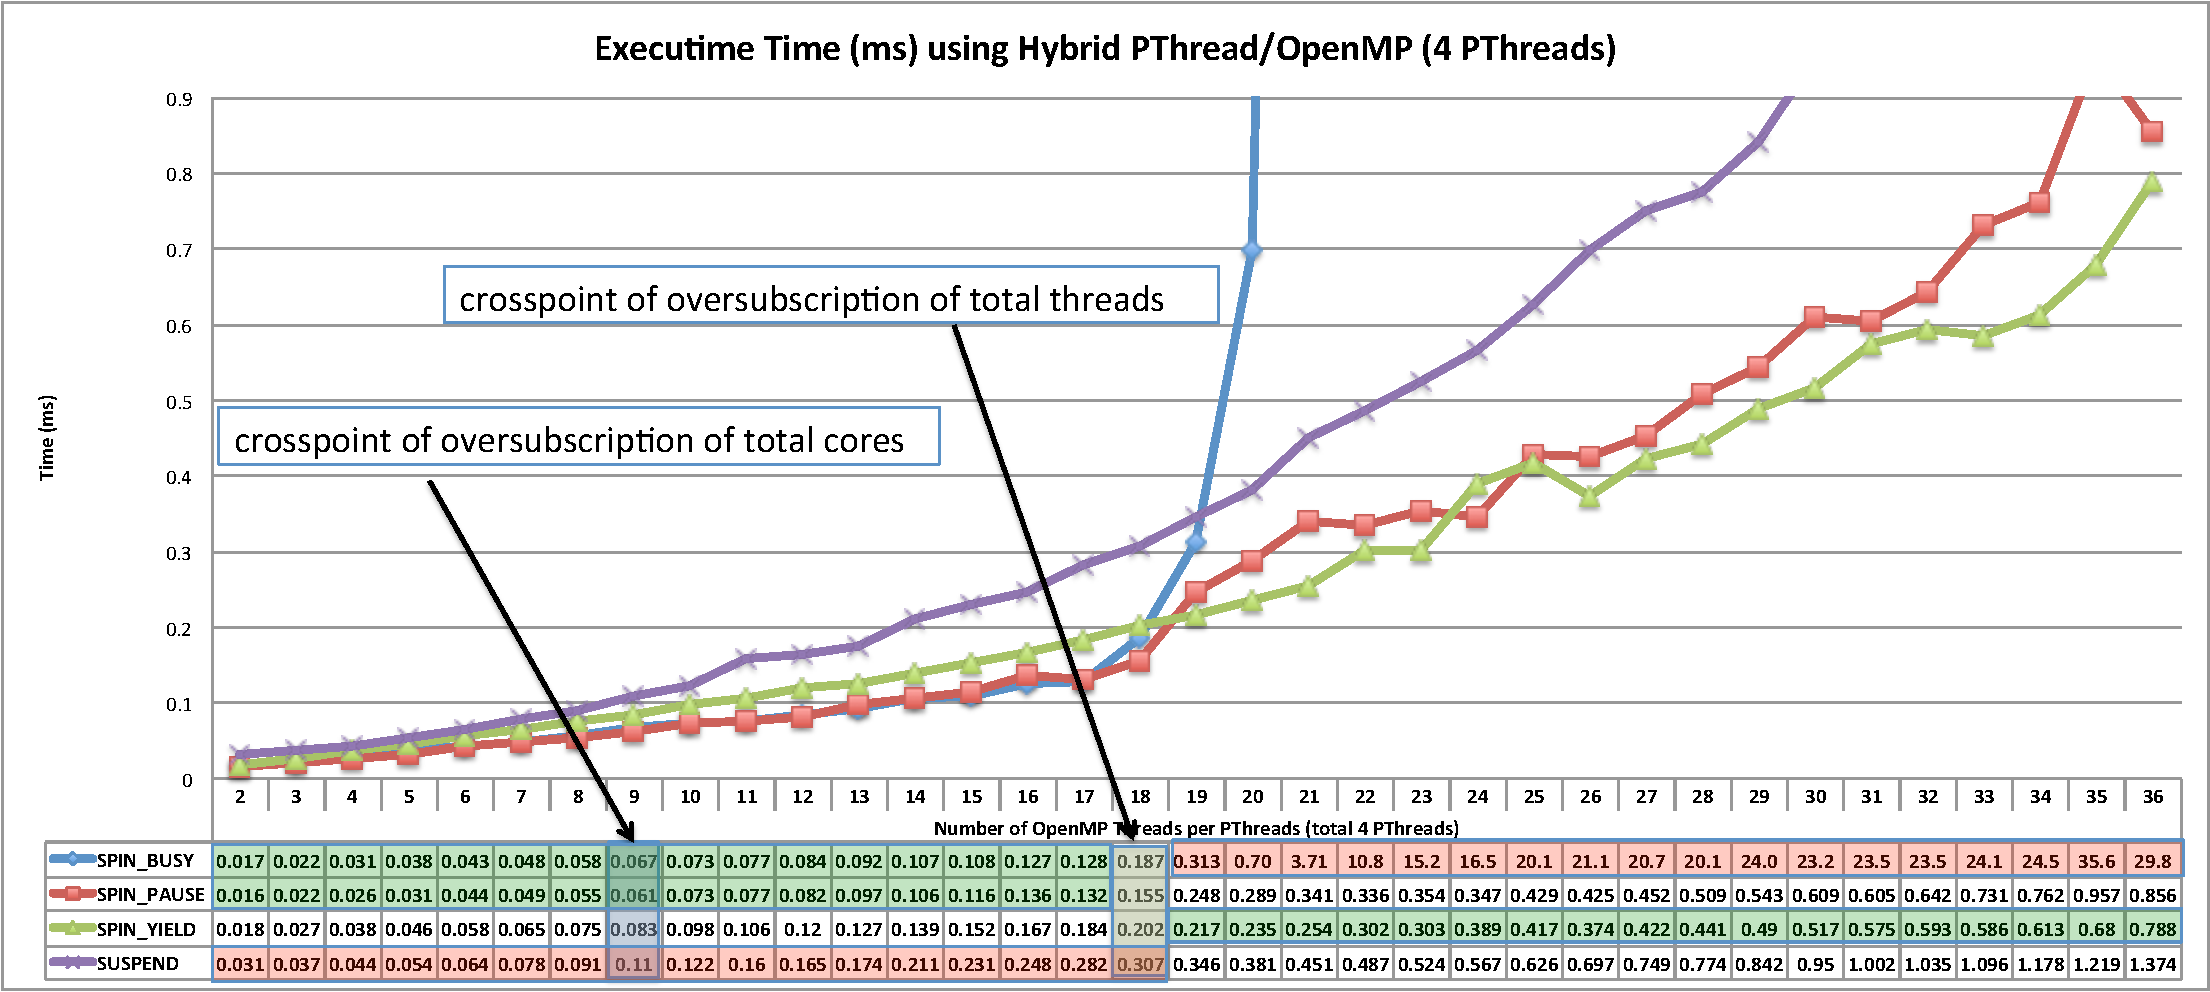
\includegraphics[width=0.99\textwidth] {images/4PThread_performance}
    \caption{Performance (ms) for hybrid PThreads/OpenMP execution: 4 PThreads and the system has total 36 cores for 72 threads.}
    \label{fig:4PThread_performance}
\end{figure}

\begin{figure}[h]
    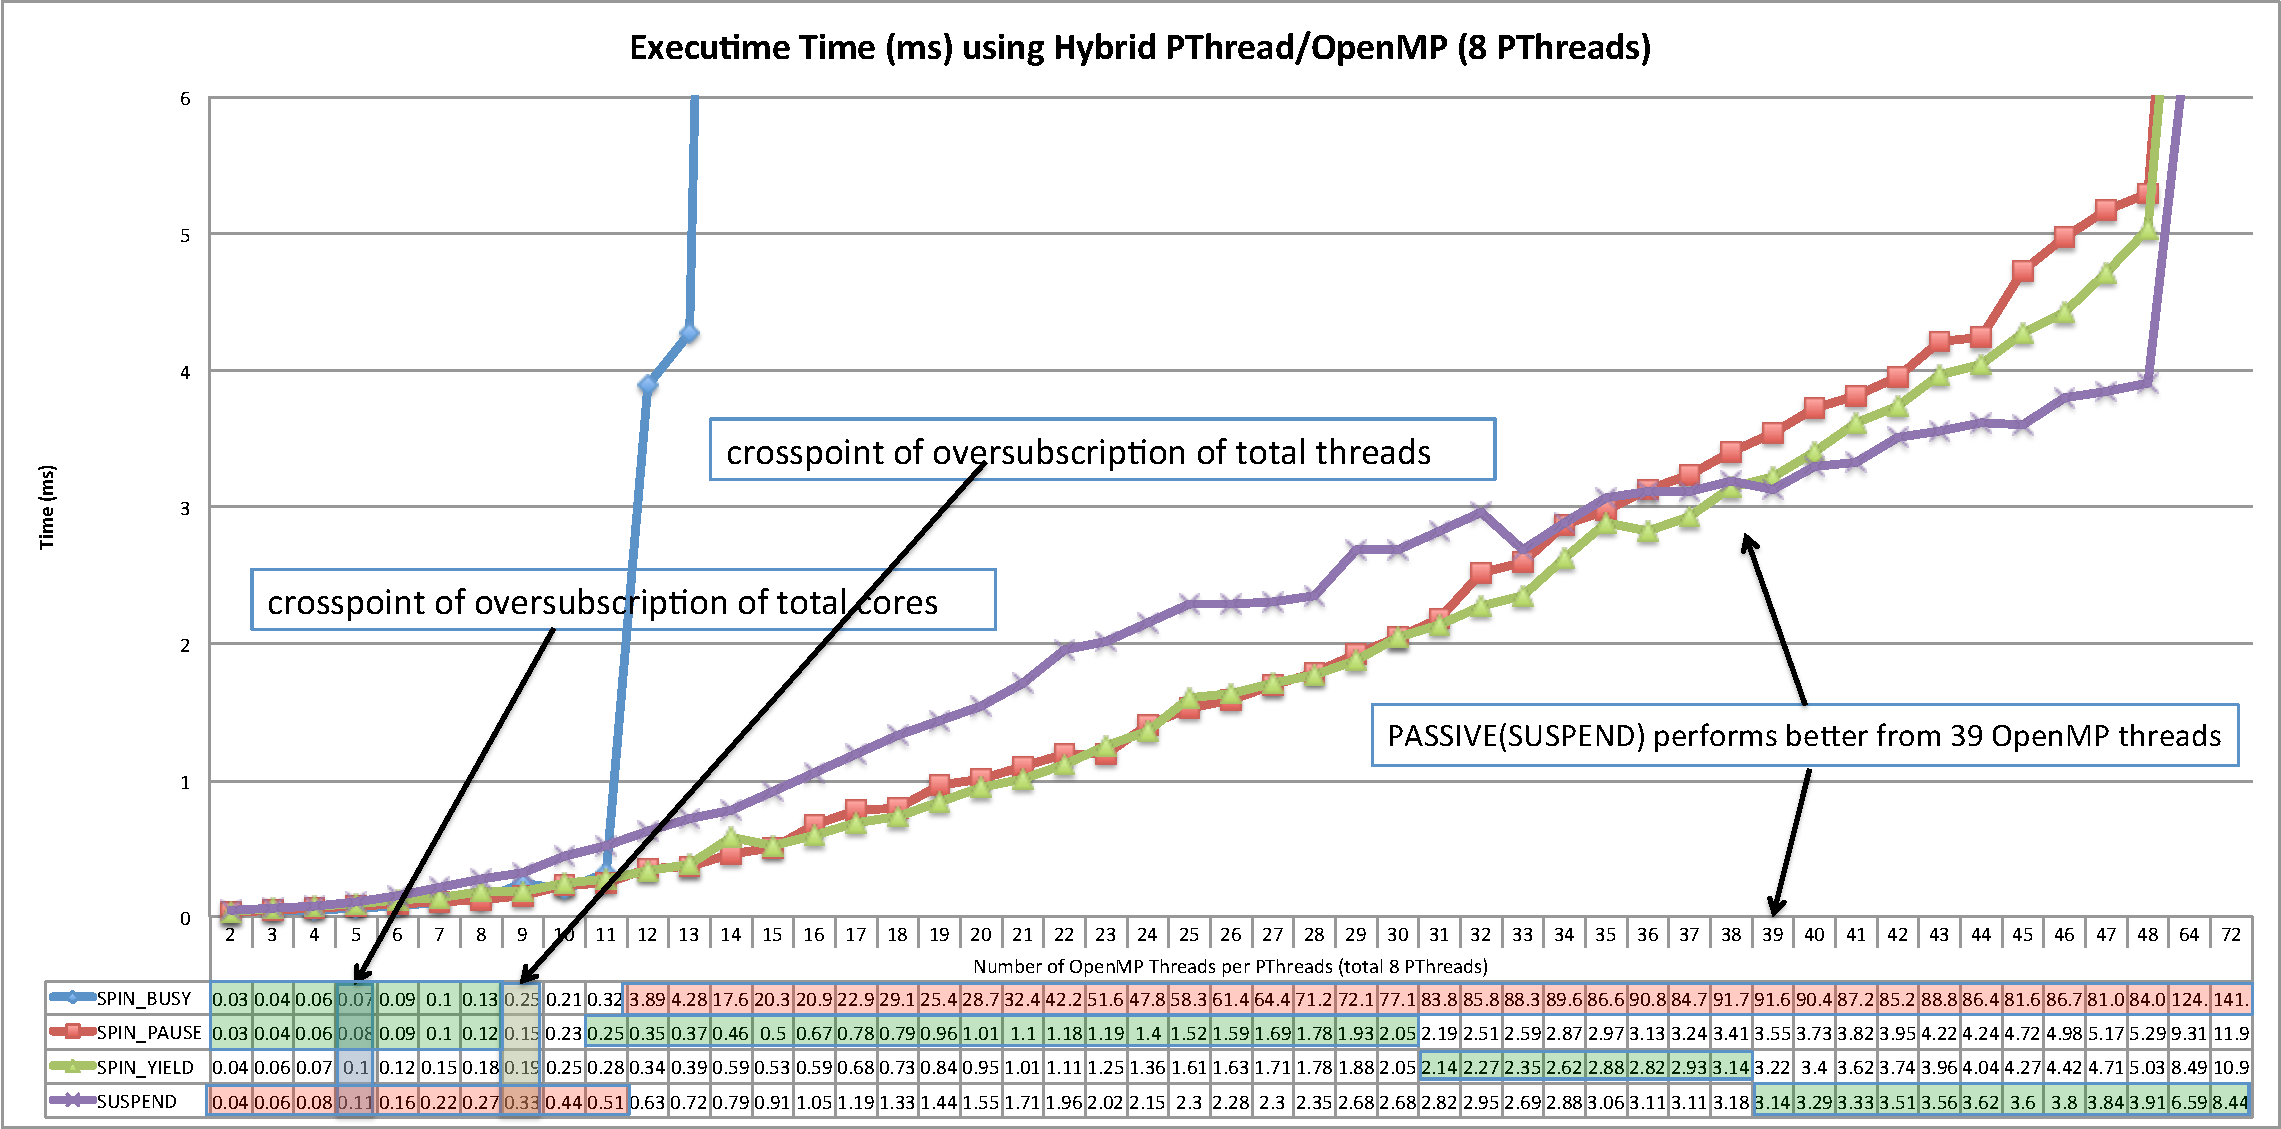
\includegraphics[width=0.99\textwidth] {images/8PThread_performance}
    \caption{Performance (ms) for hybrid PThreads/OpenMP execution: 8 PThreads and the system has total 36 cores for 72 threads.}
    \label{fig:8PThread_performance}
\end{figure}

The evaluation results using 2, 4, and 8 PThreads, each of which creates {\sf parallel} region ranging 
from 2 to 72 threads, are shown in Figure~\ref{fig:2PThread_performance},~\ref{fig:4PThread_performance} 
and~\ref{fig:8PThread_performance}. We marked the two crosspoints for each configuration in the figure and the 
policy that delivers the best performance is highilighted in green color and the worest performance in red color.
The results clearly show the effectiveness of using wait policies. For all the three configurations, 
before the crosspoint \#2 from which oversubscription just starts to occur, 
the two {\sf ACTIVE} wait polices, ({\sf SPIN\_BUSY} and {\sf SPIN\_PAUSE}, deliver the best performance and 
the {\sf PASSIVE SUSPEND} delivers the worest (max 2x time slower). 
The {\sf PASSIVE SPIN\_YIELD} delivers slightly worse performance than the two {\sf ACTIVE} policies, but still much better than the 
{\sf PASSIVE SUSPEND} policy. 
It can be explained that minumum overhead from OS kernel scheduling and context switch is incurred since 
the program does not oversubscribe the hardware threads. 
All the results also show that there are not much changes of the performance by those policies when crossing the crosspoint \#1. 
%It is very interesting that the YIELD policy performs
%consistently better than SPIN policy, indicating that even there is no oversubscription, SPIN waiting is not 
%the best option for optimal interoperability and performance.

After passing the crosspoint \#2, the results in the three figures also clearly show the dramatic increase 
of the execution time (5x to 10x) when using the {\sf ACTIVE SPIN\_BUSY} policy. 
This policy does not help address oversubscription because of the large amount of overhead from OS kernel thread scheduling and context switch 
incurred when the threads are competing for hardware cores. The mild increase
of the execution time when using either {\sf ACTIVE SPIN\_PAUSE} or {\sf PASSIVE SPIN\_YIELD} 
policy clearly shows effect of the two policies to address
the oversubscription issue. The {\sf PASSIVE SPIN\_YIELD} also performs better than {\sf ACTIVE SPIN\_PAUSE} policy. 
We also observed that the two policies consistently outperform the {\sf PASSIVE SUSPEND}
policy (20\% to 40\%) for the configuration using 2 and 4 PThreads. The 8-PThread configuration shows that the 
 {\sf PASSIVE SUSPEND} policy outperforms the other policies from 38 OpenMP threads/PThread onwards for as much as 35\%. 
 This indicates that for a program that heaviliy oversubscribes hardware resources, the {\sf PASSIVE SUSPEND} 
 policy is a better option among the four.

\subsection{Performance With Regards to the Oversubscription Ratio}
To future study the effects of the four wait policies and the approach for selecting an optimal policy for different
configurations, we introduce the term oversubscription ratio as the ratio of total number of
threads requested by a program to the total number of hardware threads. If the ratio is less than or equal to 1,
there is no oversubscription (assuming the program uses all the hardware threads of the system). 
In figure~\ref{fig:ovratio}, we consolidate the results from the previous three figures and plot with regards to 
the oversubscription ratio. The left figure shows that when the ratio is less than 1.0 (no oversubscription), 
the {\sf ACTIVE} {\sf SPIN\_BUSY} and {\sf SPIN\_PAUSE} 
deliver similar and better performance over other policies. 
When the ratio is between 1.0 to 4.0 (mild oversubscription), the {\sf ACTIVE SPIN\_PAUSE} and {\sf PASSIVE SPIN\_YIELD} policies 
perform similar and consistently better than others, but being gradualy caught up by the {\sf PASSIVE SUSPEND} policy as the ratio increases. 
The {\sf ACTIVE SPIN\_BUSY} performs very poorly right after the ratio passes 1.0. 
When the ratio is above 4.0 (heavy oversubscription), the {\sf PASSIVE SUSPEND} policy performs the best. 
\begin{figure}[h]
    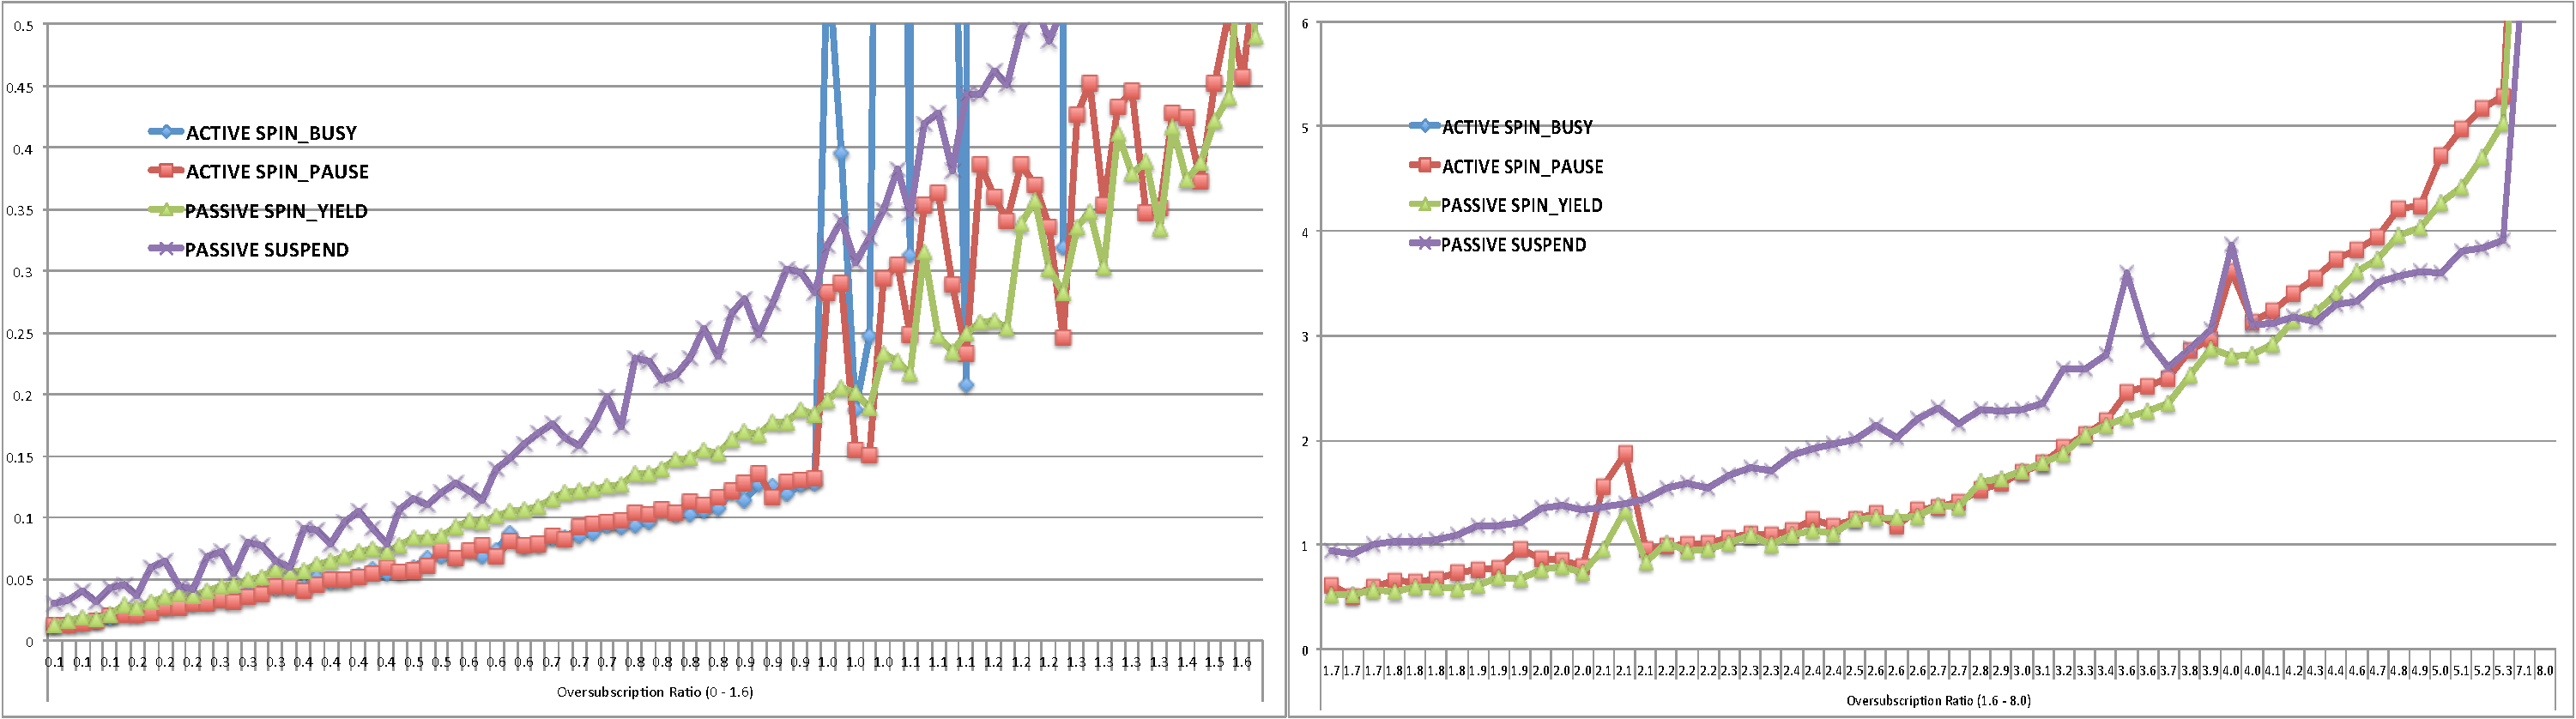
\includegraphics[width=0.99\textwidth] {images/ovratio}
    \caption{Performance (ms) of using different wait policy with regards to the oversubscription ratio}
    \label{fig:ovratio}
\end{figure}

As a summary, the evaluation demonstrates the effectiveness of the wait policy for combating the performance 
impacts of oversubscription. Heuristics for selecting the right policy 
could be drawn from this single but representative experiment as follows:
The {\sf ACTIVE SPIN\_BUSY} or {SPIN\_PAUSE} policy should be used when there is no oversubscription. 
For mild oversubscription (ratio less than 4), both {\sf ACTIVE SPIN\_PAUSE} and {\sf PASSIVE SPIN\_YIELD} are good options. 
For heavily oversubscribed system, the {\sf PASSIVE SUSPEND} policy should be 
considered to best coordinate resources between parallel runtime. 

%because the OpemMP just creates that once. Then, it puts them in a global thread pool to be used next time needed. However, the time cost represented by the quiesce term refers to the time required to shutdown the whole runtime library. In other words, after each parallel region we remove all threads in the global thread pool. Finally, the startup{\_}quiesce term implies the time required to initialize the parallel region and the time taken to shutdown the runtime library. 

% FUSED FIGURE

% ORIGINAL FIGURE
\begin{comment}
\begin{figure}[ht]
    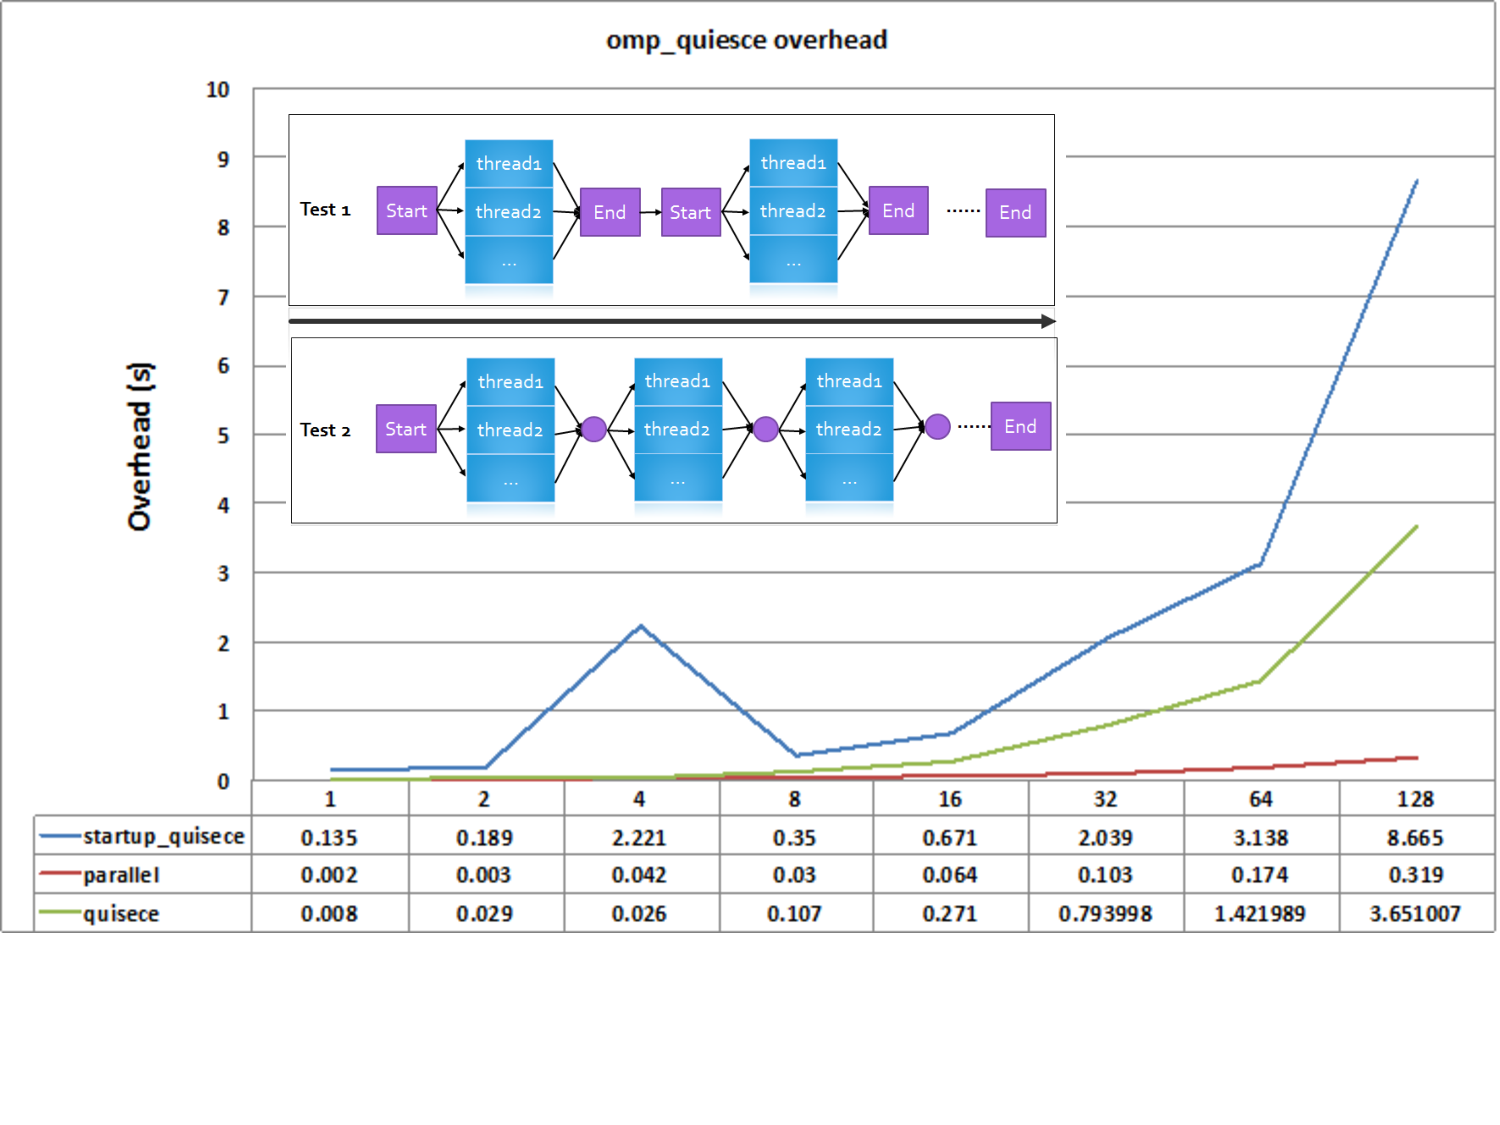
\includegraphics[width=0.9\textwidth] {images/omp_quiesce_fusion}
    \caption{{\sf omp\_quiesce} evaluation.}
    \label{omp:quiesce_evaluation}
\end{figure}
%\vspace{-0.6cm}
\begin{figure}[ht]
\subfigure[Test Design]{
		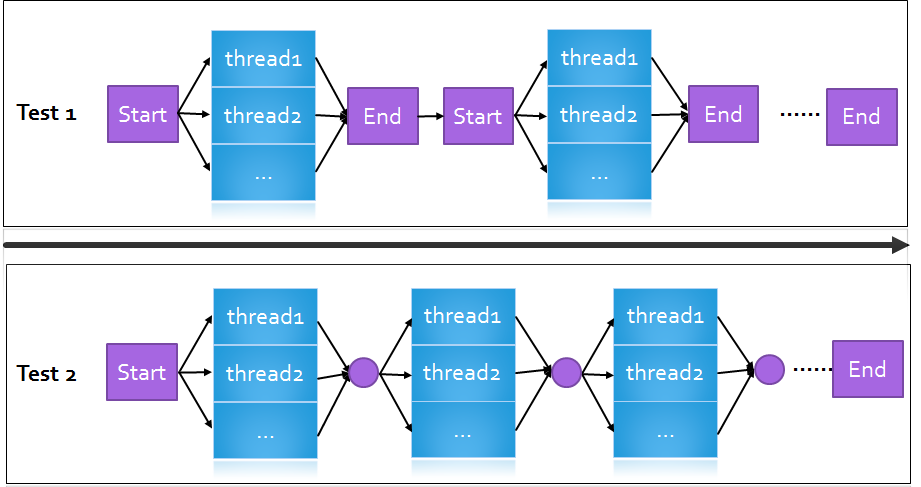
\includegraphics[width=0.6\textwidth] {images/quiesce_evaluation}
		\label{omp:quiesce_evaluation}
}
\subfigure[Evaluation Results]{
		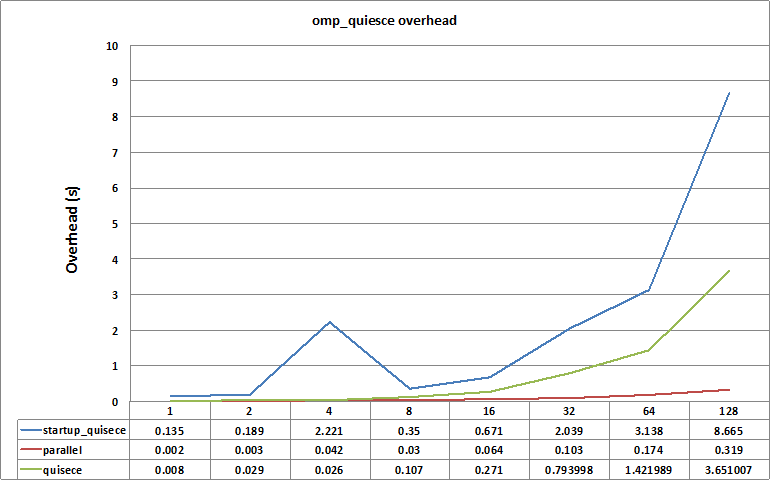
\includegraphics[width=0.6\textwidth] {images/quiesce_results}
		\label{omp:quiesce_results}
}
\caption[]{{\sf omp\_quiesce} Evaluation}
\label{fig:quiesce}
\end{figure}
%\vspace{-0.4cm}
\end{comment}


\REM{

\begin{enumerate}
	\item void omp{\_}quiesce()
	\item void omp{\_}set{\_}wait{\_}policy(PASSIVE \textbar ACTIVE)
	
	We need to create two processes since each process will only maintain and share one thread pool. For those two process, each task is execute using 1s, and we need to create enough threads to make full use of the calculation power of one CPU. We tested it in three cases: passive, active, and quiesce/restart the runtime environment. Figure~\ref{omp:wait_policy_evaluation} shows the design of the evaluation.
	
	\begin{figure}
		\centering
		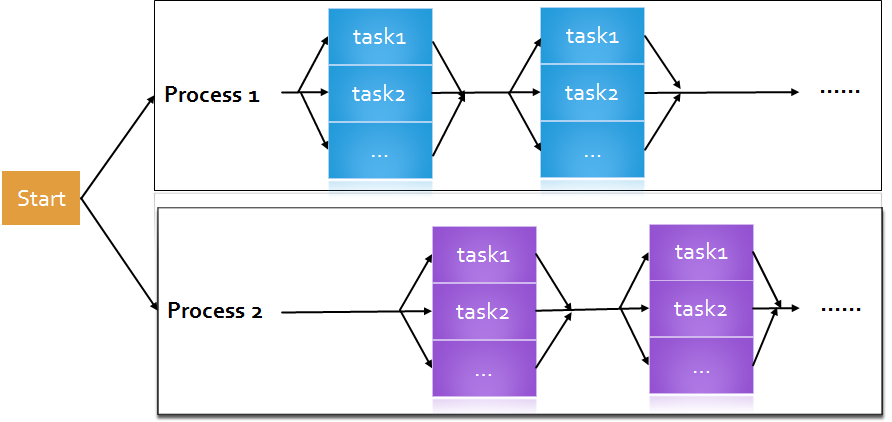
\includegraphics[width=0.7\textwidth] {images/wait_policy_evaluation}
		\caption{waiting policy evaluation}
		\label{omp:wait_policy_evaluation}
	\end{figure}
	
	As Figure~\ref{omp:wait_policy_results} below shows, there is no a big difference between the two behaviors. The reason is that the OpenMP uses only one global thread pool for all OpenMP threads created by multiple PThreads. So, the small difference comes from the time required to awake a sleeping thread. By doing this experiment, we have understand more about the way that OpenMP deals with the thread pool. 
	
	\begin{figure}
		\centering
		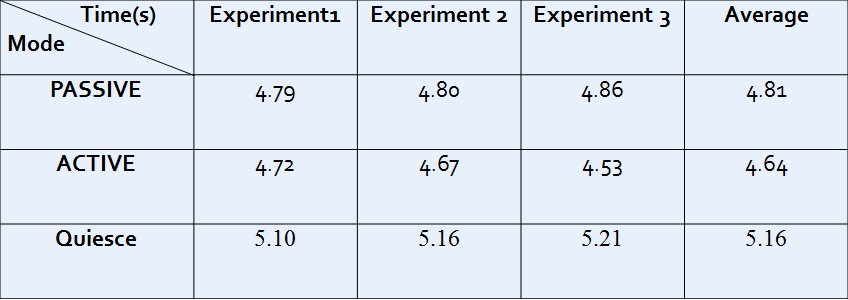
\includegraphics[width=0.7\textwidth] {images/wait_policy_results}
		\caption{Waiting Policy Results}
		\label{omp:wait_policy_results}
	\end{figure}
	
	
	\item int omp{\_}thread{\_}create()
	
	We compared this function with creating pthread to execute a list of tasks. So, for this function we have tested it in two different ways. Figure~\ref{omp:create_evaluation} shows the design of the evaluation. For the first way, we put different number of tasks in one parallel region, so that every “omp{\_}thread{\_}create()” or “pthread{\_}create()” function will be run in parallel. On the other hand, we use different iterations to execute the “omp{\_}thread{\_}create()” or “pthread{\_}create()” functions in sequence, and compare the running time. 
	
	\begin{figure}
		\centering
		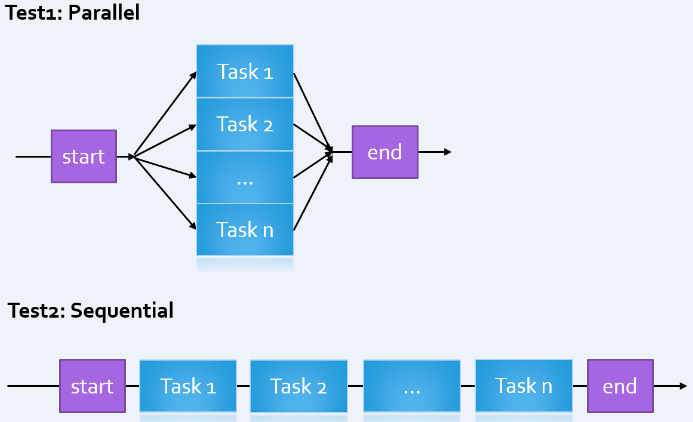
\includegraphics[width=0.7\textwidth] {images/create_evaluation}
		\caption{creating thread evaluation}
		\label{omp:create_evaluation}
	\end{figure}
	
	Figure~\ref{omp:create_results_parallel2} and Figure~\ref{omp:create_results_parallel} show the result of the first approach (execute in parallel). It clearly shows that there is almost no differences between them. This is might be because that we are doing it inside the parallel region.However, Figure~\ref{omp:create_results_sequence2} and Figure~\ref{omp:create_results_sequence} show the result of the second approach (execute in sequence). They show that omp{\_}thread{\_}create() gives a better performance that pthread{\_}create( ). So, it would be a good feature if the user can do this instead of creating another pthread.

% I do not think we need these.  The performance should be relatively obvious
% and in any case should not matter.  The purpose is to create an OS thread
% that the OpenMP runtime is aware of, and otherwise it should be the thinnest
% possible wrapper about the native OS thread library.
% Because of this, I do not see how omp_thread_create can be faster than
% pthread_create.
%                       - Jeff
\begin{comment}
	\begin{figure}
		\centering
		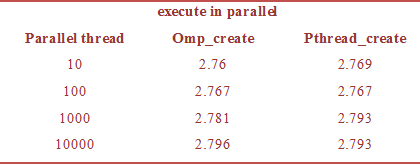
\includegraphics[width=0.7\textwidth] {images/create_results_parallel2}
		\caption{Results of omp\_thread\_create in parallel}
		\label{omp:create_results_parallel2}
	\end{figure}
	\begin{figure}
		\centering
		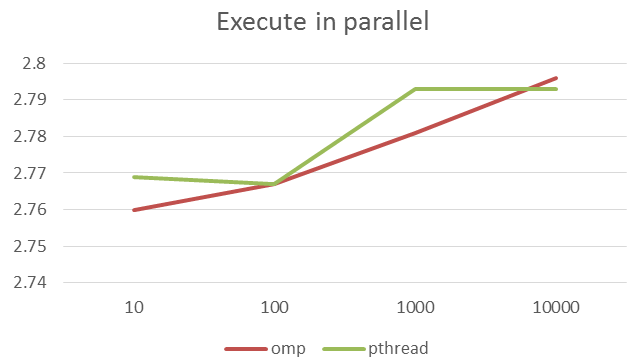
\includegraphics[width=0.7\textwidth] {images/create_results_parallel}
		\caption{Results of omp\_thread\_create in parallel}
		\label{omp:create_results_parallel}
	\end{figure}
	\begin{figure}
		\centering
		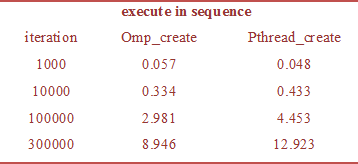
\includegraphics[width=0.7\textwidth] {images/create_results_sequence2}
		\caption{Results of omp\_thread\_create in sequence}
		\label{omp:create_results_sequence2}
	\end{figure}
	\begin{figure}
		\centering
		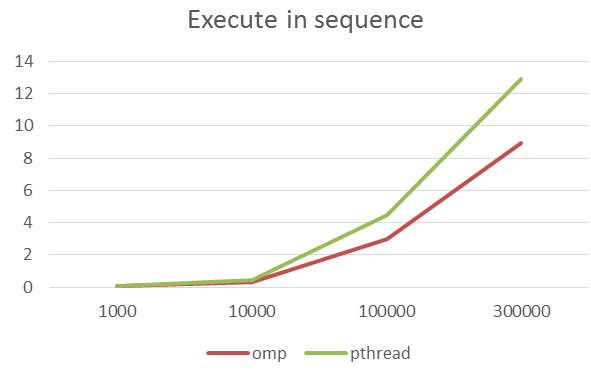
\includegraphics[width=0.7\textwidth] {images/create_results_sequence}
		\caption{Results of omp\_thread\_create in sequence}
		\label{omp:create_results_sequence}
	\end{figure}
\end{comment}

\end{enumerate}

}


